\documentclass[12pt,a4paper]{article}

% --- Paquetes básicos ---
\usepackage[utf8]{inputenc}     % Acentos
\usepackage[T1]{fontenc}
\usepackage[spanish,es-tabla]{babel}     % Idioma
\usepackage{geometry}           % Márgenes
\usepackage{graphicx}           % Imágenes
\usepackage{float}              % Posición exacta de figuras
\usepackage{hyperref}           % Hipervínculos
\usepackage[table]{xcolor}      % Colores (con table para \rowcolor)
\usepackage{fancyhdr}           % Encabezados y pies de página
\usepackage{titlesec}           % Formato de títulos
\usepackage{listingsutf8}       % Soporte UTF-8 en listing
\usepackage{listings}           % Código
\usepackage{caption}            % Personalizar captions
\usepackage{amsmath, amssymb}   % Símbolos matemáticos
\usepackage{booktabs}           % Tablas elegantes
\usepackage{array}              % Columnas sin justificar en tablas
\usepackage{longtable}
\usepackage{seqsplit}
\usepackage[printonlyused]{acronym}  % Acrónimos: se desarrollan solo la primera vez
\usepackage{multirow}

\emergencystretch=3em   % evita líneas que se salen del margen

\addto\captionsspanish{
  \renewcommand{\tablename}{Tabla}
  \renewcommand{\contentsname}{Tabla de contenidos}
}

% Cambios respecto al entregable 1 (el enunciado pide resaltarlos claramente).
% Uso: \cambio{texto modificado}. Sale en azul en el PDF.
\newcommand{\cambio}[1]{\textcolor{blue}{#1}}

% --- Configuración de códigos ---
\lstset{
  basicstyle=\ttfamily\small,
  backgroundcolor=\color{gray!10},
  frame=single,
  breaklines=true,
  columns=fullflexible,
  inputencoding=utf8,
  extendedchars=true,
  literate=
    {á}{{\'a}}1 {é}{{\'e}}1 {í}{{\'i}}1 {ó}{{\'o}}1 {ú}{{\'u}}1
    {Á}{{\'A}}1 {É}{{\'E}}1 {Í}{{\'I}}1 {Ó}{{\'O}}1 {Ú}{{\'U}}1
    {ñ}{{\~n}}1 {Ñ}{{\~N}}1
}

% Estilo para Scala
\lstdefinestyle{miEstiloScala}{
    language=Scala,
    basicstyle=\small\ttfamily,
    backgroundcolor=\color{gray!5},
    keywordstyle=\color{blue}\bfseries,
    commentstyle=\color{green!60!black}\itshape,
    stringstyle=\color{red},
    showstringspaces=false,
    frame=single,
    breaklines=true,
    captionpos=b,
    morekeywords={val, var, def, class, object, trait, extends, with, match, case, new, if, else, for, while, return, type, import, package}
}

% --- Configuración de márgenes ---
\geometry{top=2.5cm, bottom=2.5cm, left=3cm, right=2.5cm}

% --- Configuración de hipervínculos ---
\hypersetup{
    colorlinks=true,
    linkcolor=black,   % índices y referencias a secciones, tablas y figuras
    citecolor=black,   % citas [1], [2]...
    urlcolor=cyan      % enlaces web
}

% --- Encabezados y pies de página ---
\pagestyle{fancy}
\fancyhf{}
\fancyhead[L]{Universidad de Valladolid}
\fancyhead[R]{Máster en Ingeniería Informática}
\fancyfoot[C]{\thepage}

% --- Formato de títulos ---
\titleformat{\section}[hang]{\bfseries\Large}{\thesection}{1em}{}

% -- Información para la portada
\title{\LARGE \textbf{Proyecto de Clasificación: Tercera Etapa}\\[0.3cm]
\large \textbf{Creación, selección y evaluación de modelos}}
\author{{\large \textbf{Autores:}}\\[0.10cm]
    Gonzalo Agúndez Sáez \\
    Paula Negro Asegurado \\
    Diego Sanz Santos }
\date{\normalsize \today}

\makeatletter
\let\thetitle\@title
\let\theauthor\@author
\let\thedate\@date
\makeatother

\begin{document}

\begin{titlepage}
    \centering
    \vspace*{0.5cm}
    
\includegraphics[width=0.65\textwidth]{logoInfo.png}\\[0.8cm]

    {\Huge \bfseries \thetitle}\\[1.0cm]

    {\Large \bfseries Asignatura: Técnicas escalables de análisis de datos (Clasificadores)}\\[0.3cm]
    {\large Escuela de Ingeniería Informática}\\[0.8cm]

    \theauthor \\[0.5cm]
    Grupo 3 -- Conjunto de datos 2 (\textit{NYC Taxi Trip Duration}) \\[0.3cm]
    \textbf{Curso:} 2026 -- 2027 \\[0.3cm]
    \textbf{Fecha:} \thedate

    \vfill
    \rule{0.5\linewidth}{0.5pt}\\
    \textit{Universidad de Valladolid}
\end{titlepage}

\tableofcontents
\clearpage
\listoffigures    % Índice de imágenes
\listoftables     % Índice de tablas

% =====================================================================
% ACRÓNIMOS: \ac{X} en el texto (la primera vez sale desarrollado);
% \acs{X} en tablas, fórmulas y pies (solo la sigla).
% Con printonlyused solo aparecen los que se usan al menos una vez.
% =====================================================================
\section*{Acrónimos}

\begin{acronym}[NTAIE]
  \acro{DT}{árbol de decisión}
  \acro{FN}{falso negativo}
  \acro{FP}{falso positivo}
  \acro{NTAIE}{número total de ausentes o inconsistentes eliminados}
  \acro{NTOE}{número total de \textit{outliers} eliminados}
  \acro{PR}{precisión--exhaustividad}
  \acro{RF}{\textit{Random Forest}}
  \acro{ROC}{característica operativa del receptor}
  \acro{TN}{verdadero negativo}
  \acro{TP}{verdadero positivo}
\end{acronym}

\newpage
% =====================================================================
\section{Introducción}
% =====================================================================

Este trabajo corresponde a la tercera etapa del proyecto de clasificación en Spark. Su objetivo es crear, seleccionar y evaluar dos modelos finales que clasifiquen los viajes del conjunto \textit{New York City Taxi Trip Duration} según su duración en tres clases: \textit{short} (hasta 10 minutos), \textit{medium} (hasta 25) y \textit{long} (más de 25). Es, por tanto, un problema de clasificación multiclase. A diferencia de lo que se proponía en el entregable individual, donde se permitía convertir el problema en binario, aquí se mantienen las tres clases, para que el problema sea el mismo que el planteado en el primer entregable.\\

De los dos modelos, al menos uno tiene que ser un clasificador avanzado, y
el otro puede ser básico. Se han elegido dos modelos de Spark ML:
\begin{itemize}
    \item un \textbf{\ac{DT}}, como modelo básico
    (sección~\ref{sec:seleccion-dt});
    \item un \textbf{\ac{RF}}, como modelo avanzado
    (sección~\ref{sec:seleccion-rf}). Combina muchos árboles para reducir el
    sobreajuste de uno solo y admite directamente las tres clases, a
    diferencia de otros modelos de Spark, como los \textit{Gradient-Boosted
    Trees}, que solo admiten clasificación binaria.
\end{itemize}
Uno de los objetivos es comparar cómo se comportan dos modelos distintos con
los mismos datos: si el modelo avanzado mejora de verdad al básico y a qué
coste\\

Respecto al primer entregable, \cambio{que hemos actualizado y enviado junto
con este documento,} se revisan la limpieza y la transformación: se eliminan
muchos menos viajes y cambia el cálculo de la distancia. Para seleccionar
los parámetros de cada modelo se usan las utilidades de Spark ML
(\texttt{ParamGridBuilder} y \texttt{CrossValidator}), con validación
cruzada y una búsqueda en dos fases: primero una rejilla gruesa, con valores
muy separados, y después una fina alrededor de los mejores.\\

La sección~\ref{sec:resumen} resume el conjunto de datos. La sección~\ref{sec:trabajo} describe el trabajo realizado: los conjuntos de entrenamiento y prueba, la limpieza y la transformación revisadas, la creación y selección de cada modelo y su evaluación sobre el conjunto de prueba.


% =====================================================================
\section{Resumen ejecutivo del conjunto de datos}
\label{sec:resumen}
% =====================================================================

\begin{itemize}
    \item \textbf{Origen de los datos:} competición de Kaggle \textit{New York City Taxi Trip Duration}, basada en los registros de taxis amarillos de Nueva York de 2016 publicados por la NYC Taxi and Limousine Commission (TLC), el organismo municipal que regula los taxis y vehículos de alquiler de la ciudad. Se utiliza el fichero \texttt{train.csv}, disponible en \url{https://www.kaggle.com/c/nyc-taxi-trip-duration/data}.
    \item \textbf{Propósito:} el propósito original es predecir la duración de un viaje en taxi a partir de sus atributos (fecha y hora, coordenadas, pasajeros, etc.). En este proyecto se plantea como un problema de \textbf{clasificación multiclase}: predecir si un viaje es corto, medio o largo.
    \item \textbf{Tamaño:} 1\,458\,644 instancias y 11 atributos originales, sin valores ausentes ni duplicados.
    \item \textbf{Atributos (11 en total):}
    \begin{itemize}
        \item \textbf{Nominales (4):} \texttt{id} (identificador único del viaje), \texttt{vendor\_id} (proveedor del registro: 1 o 2) y las marcas temporales \texttt{pickup\_datetime} y \texttt{dropoff\_datetime}.
        \item \textbf{Numéricos continuos (5):} \texttt{pickup\_longitude}, \texttt{pickup\_latitude}, \seqsplit{\texttt{dropoff\_longitude}}, \texttt{dropoff\_latitude} y \texttt{trip\_duration} (en segundos).
        \item \textbf{Numéricos discretos (1):} \texttt{passenger\_count} (de 0 a 9).
        \item \textbf{Booleanos (1):} \texttt{store\_and\_fwd\_flag} (Y/N).
    \end{itemize}
    \item \textbf{Descripción de la clase:} se construye a partir de \texttt{trip\_duration}, que se descarta como atributo predictor. Tiene tres valores: \textit{short} (duración $\leq$ 10 min), \textit{medium} (entre 10 y 25 min) y \textit{long} ($>$ 25 min). En el conjunto original, el reparto es \textit{short} 44,76\,\%, \textit{medium} 42,87\,\% y \textit{long} 12,37\,\%. \cambio{Con la limpieza revisada, el conjunto de entrenamiento queda en 44,85 / 42,89 / 12,26\,\%.} \textit{Long} es una minoría clara, lo que supone un desequilibrio moderado entre clases.
\end{itemize}


% =====================================================================
\section{Descripción del trabajo realizado}
\label{sec:trabajo}
% =====================================================================

Esta sección sigue las fases del proyecto. Las tres primeras (conjuntos,
limpieza y transformación) preparan los datos y parten del primer
entregable: se resume lo que se mantiene y se detallan las correcciones,
que aparecen \cambio{en azul}. Las dos últimas aprovechan esos datos ya
preparados para crear y seleccionar los modelos y, después, evaluarlos.

\subsection{Conjuntos de entrenamiento y prueba}
\label{sec:conjuntos}

Se mantiene la partición del primer entregable: un 80\,\% para entrenamiento y un 20\,\% para prueba, con \texttt{randomSplit} y semilla 42, hecha sobre el conjunto completo antes de limpiar. Como la limpieza se aplica después, cambiarla no altera la partición.

\begin{table}[H]
\centering
\small
\begin{tabular}{lrrrr}
\toprule
\textbf{Conjunto} & \textbf{Instancias} & \textbf{\textit{short} (\%)} & \textbf{\textit{medium} (\%)} & \textbf{\textit{long} (\%)} \\
\midrule
Original      & 1\,458\,644 & 44,76 & 42,87 & 12,37 \\
Entrenamiento & 1\,166\,855 & 44,79 & 42,84 & 12,37 \\
Prueba        &   291\,789 & 44,63 & 42,98 & 12,38 \\
\bottomrule
\end{tabular}
\caption{Tamaño y reparto de la clase de cada conjunto, antes de limpiar.}
\label{tab:particion}
\end{table}

El conjunto de entrenamiento se usa para crear los modelos y seleccionar sus parámetros mediante validación cruzada. El de prueba no interviene en ninguna decisión: solo se usa una vez, al final, para evaluar los modelos finales. La partición aleatoria conserva el reparto de la clase (\textit{long} es el 12,37\,\% en entrenamiento y el 12,38\,\% en prueba), así que no hace falta estratificar.

\subsection{Limpieza de datos}
\label{sec:limpieza}

En el primer entregable se eliminaban los viajes con pasajeros fuera de 1--6, con coordenadas fuera de un rectángulo amplio alrededor de Nueva York, de 0 km con más de 5 minutos, de menos de 60 s y de más de 3 h. En total se descartaba el 0,956\,\% de los datos y el 1,00\,\% del conjunto de prueba. Al revisar esos criterios se ha considerado que varios eran demasiado estrictos: eliminaban viajes raros pero posibles, y un 1\,\% de no clasificados es una pérdida de datos excesiva.

\cambio{Por eso se cambia el criterio general: \textbf{solo se eliminan los registros imposibles}. Los valores raros pero posibles se mantienen, porque son viajes reales y el modelo tiene que saber clasificarlos. Además, filtrar por duración es filtrar por la etiqueta, y con datos nuevos la duración no se conoce, así que ese filtro se reduce al mínimo.} A continuación se explica cada cambio; la tabla~\ref{tab:atributos}, al final de la sección, los resume todos.

\paragraph{Pasajeros.} En el primer entregable se eliminaban los viajes con 0 pasajeros o con 7 a 9. \cambio{Son poco habituales, pero no imposibles: un viaje con 0 pasajeros puede ser un envío de paquetes, y uno de 7 a 9, una limusina o un vehículo de mayor capacidad. Su duración se registra igual que la de cualquier otro, así que su clase es correcta. Por eso se mantienen.}

\paragraph{Viajes de 0 km.} En el primer entregable, los 3\,191 viajes de 0 km y más de 5 minutos se eliminaban porque contradicen a la distancia, el atributo que mejor separa las clases: un viaje sin desplazamiento debería ser corto, y si dura más de 5 minutos el modelo recibe un ejemplo que va en contra de esa regla. \cambio{Sin embargo, que la distancia registrada sea 0 no significa que el viaje no exista. Puede deberse a un atasco, con el taxi casi parado durante muchos minutos, algo habitual en el tráfico de Nueva York, o a que se registró como destino la misma dirección de recogida, por ejemplo en un viaje de ida y vuelta. En ambos casos la duración es real y su clase es correcta. Eliminarlos quitaría al modelo viajes que también aparecerán con datos nuevos, así que se mantienen: el modelo que se elija tendrá que aprender que, en esos casos, la distancia no es suficiente y decidir con el resto de atributos.}

\paragraph{Duración.} En el primer entregable se eliminaban los viajes de menos de 60 s, porque un viaje real de menos de un minuto se consideró poco creíble, y los de más de 3 h, porque ese corte separaba el bloque anómalo de unas 24 h de los viajes largos normales y porque se consideró que un viaje de más de 3 horas era algo raro. \cambio{Al revisarlo, los dos cortes resultan demasiado estrictos. Las clases se definen solo a partir de la duración (\textit{short} hasta 10 minutos, \textit{medium} hasta 25 y \textit{long} a partir de ahí). Por eso, aunque un viaje de 30 s o de 5 h tenga una duración extrema, su etiqueta es correcta: el de 30 s es \textit{short} y el de 5 h es \textit{long}. En escala logarítmica (figura~\ref{fig:logduracion}), por debajo de 60 s la distribución baja poco a poco, sin un salto, y entre 3 y 23 h solo hay 269 viajes, todos \textit{long} (como se vio en el entregable anterior): es el final normal de la distribución. Además, en Nueva York no es raro que un taxi tarde varias horas, por ejemplo en un viaje fuera de la ciudad o con mucho tráfico, así que estos viajes se mantienen. En cambio, los 1\,843 viajes de más de 23 h forman un pico aislado en torno a las 24 h, separado del resto. Por eso se consideran registros fallidos; una posible explicación, que no se puede comprobar con estos datos, es un taxímetro que no se apagó al terminar el viaje. Si es así, su duración real es desconocida y su etiqueta no es fiable, así que se eliminan.}

\begin{figure}[H]
\centering
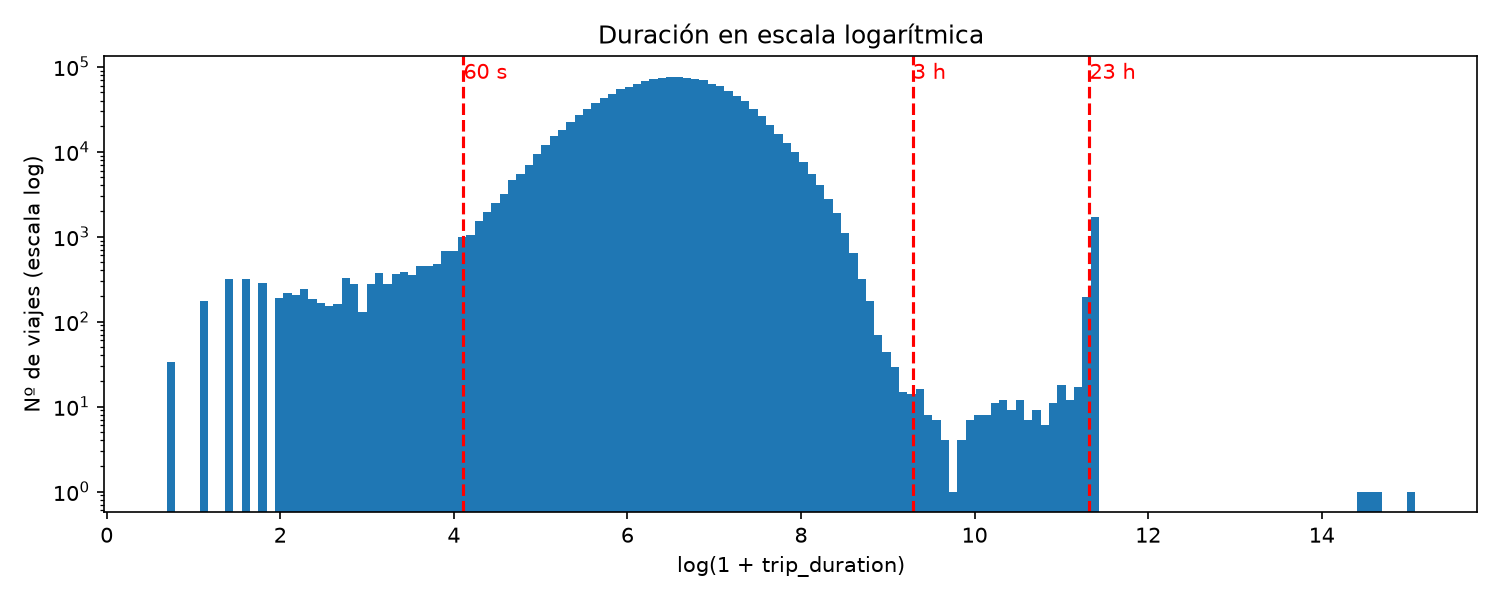
\includegraphics[width=0.9\textwidth]{diagramas/histograma_log_duracion.png}
\caption{Duración de los viajes en escala logarítmica (también en el eje vertical), con los cortes de 60 s, 3 h y 23 h.}
\label{fig:logduracion}
\end{figure}

\paragraph{Coordenadas.} Para las coordenadas se usan dos rectángulos, como en el primer entregable. El \textbf{rectángulo ajustado} a la ciudad (latitud 40,477--40,917; longitud $-74{,}256$ a $-73{,}7$) solo sirve de referencia para ver qué viajes salen de Nueva York, y no elimina nada. El \textbf{rectángulo amplio} (latitud 40,0--41,5; longitud $-74{,}8$ a $-73{,}0$) marca el límite de lo imposible: lo que queda fuera está a cientos de kilómetros (hasta longitud $-121{,}93$), y esos viajes sí se eliminan. La figura~\ref{fig:rectangulos} muestra los dos.

\cambio{En el primer entregable se indicó que quedaban fuera del rectángulo amplio 81 viajes, pero esa cifra era la suma de 35 recogidas y 46 destinos. Como 32 viajes tienen las dos coordenadas fuera, se contaron dos veces: en realidad son 49 viajes distintos.} \cambio{Los viajes que salen del rectángulo ajustado se mantienen: sus destinos tienen una distancia mediana de 22,6 km y una duración mediana de 34 min, frente a 2,1 km y 11 min de los de dentro, y el 67,8\,\% son \textit{long}, así que son viajes largos reales. Las recogidas de fuera también son posibles, por ejemplo un taxi que deja a un cliente fuera de la ciudad y recoge allí mismo al siguiente.}

\begin{figure}[H]
\centering
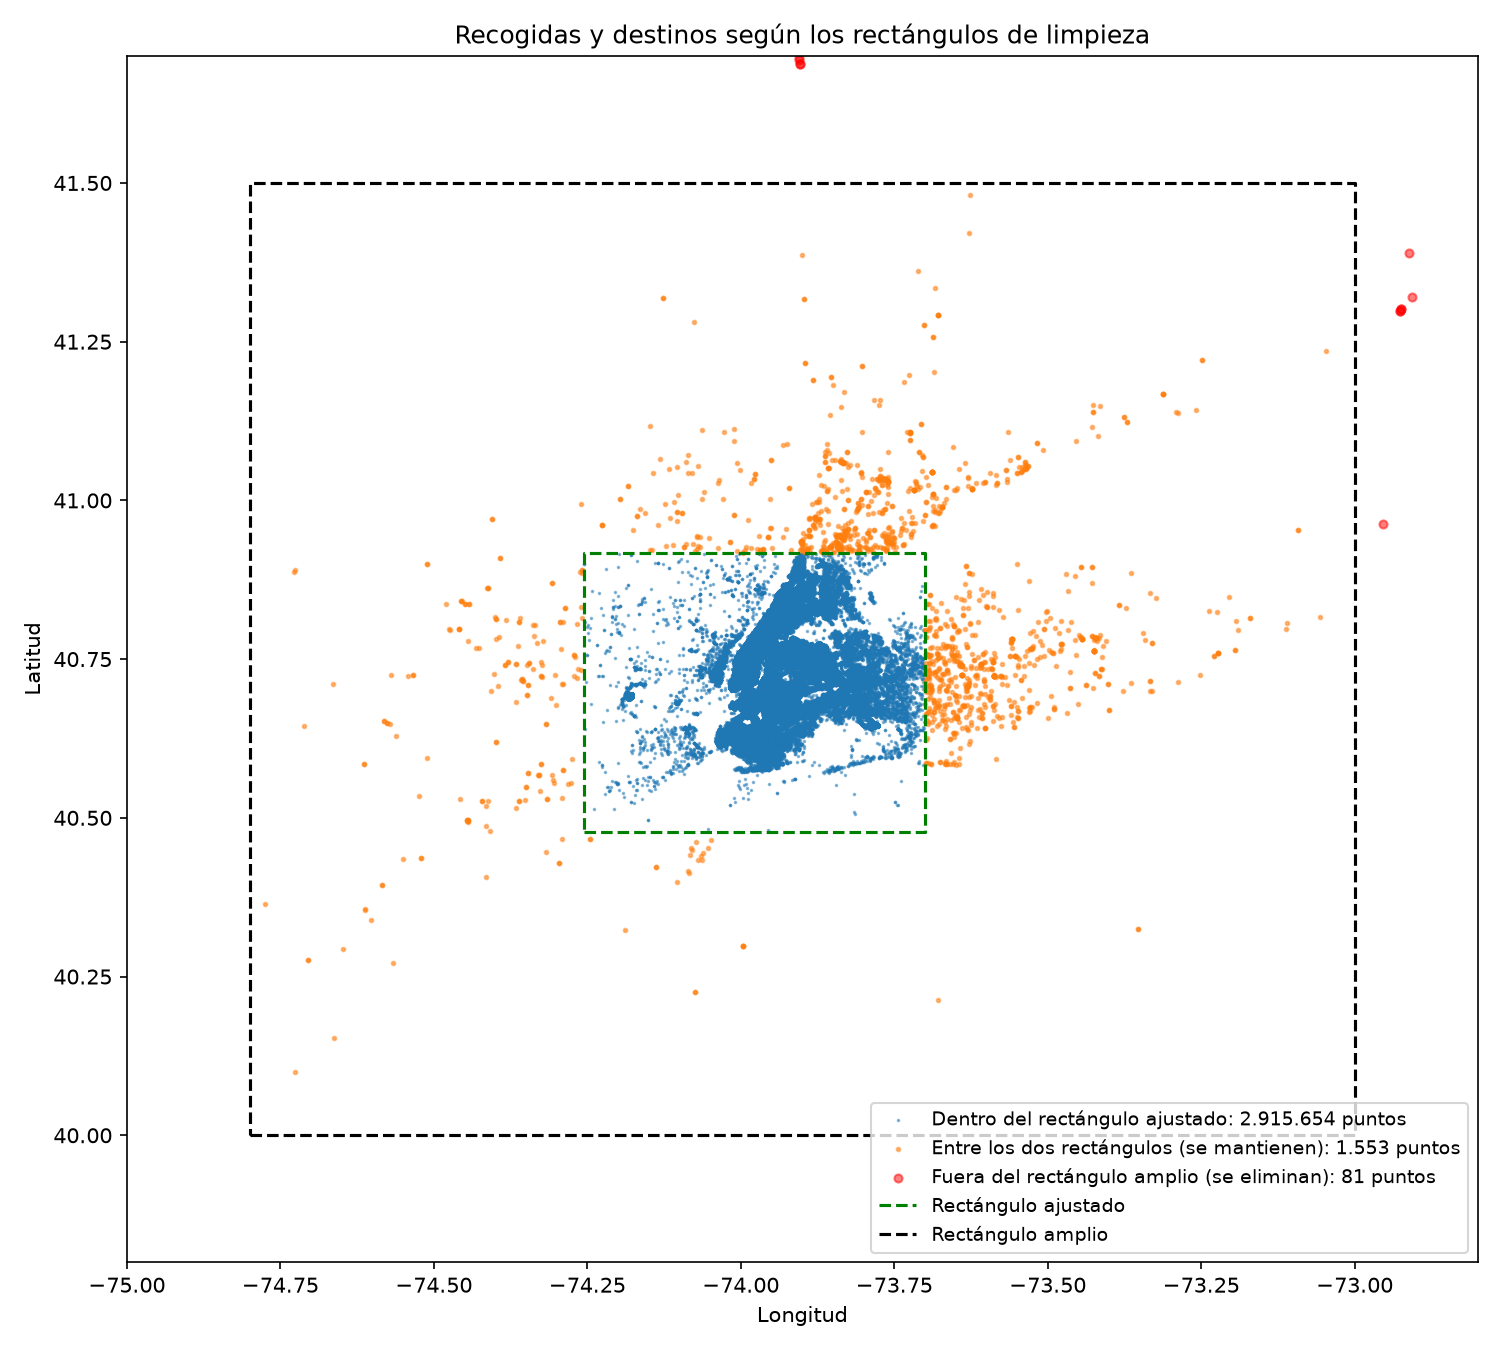
\includegraphics[width=0.8\textwidth]{diagramas/mapa_rectangulos.png}
\caption{Recogidas y destinos según el rectángulo en el que caen. Cada viaje aporta dos puntos, así que los 81 puntos rojos corresponden a 49 viajes; los más lejanos quedan fuera de la vista.}
\label{fig:rectangulos}
\end{figure}

\cambio{Por último, algunos puntos de recogida o destino caen sobre el río. Ningún rectángulo los detecta, porque están dentro de la ciudad, y eliminarlos con precisión exigiría la forma exacta de la costa, algo que no se puede aplicar en la limpieza con un criterio sencillo como el de los rectángulos. Además, no tiene por qué tratarse de errores en el viaje: pueden deberse a la imprecisión del GPS cerca de la orilla o a los túneles que pasan bajo el río (Holland, Lincoln y Queens-Midtown), en los que un taxi aparece sobre el agua aunque circule con normalidad. La duración de esos viajes es real, así que su clase es correcta. Por eso se mantienen; además, en el mapa se aprecia que son muy pocos frente a los casi tres millones de puntos, así que su efecto en el modelo es despreciable.}

\paragraph{Resultado.} La limpieza se aplica con la misma función a entrenamiento y a prueba. En prueba, las filas eliminadas se cuentan como \ac{NTAIE} (coordenadas imposibles) o \ac{NTOE} (más de 23 h); si una fila cumple los dos criterios, cuenta como \acs{NTAIE}. La tabla~\ref{tab:limpieza} compara el resultado con el del primer entregable.

\begin{table}[H]
\centering
\small
\begin{tabular}{lrr}
\toprule
 & \textbf{Entregable 1} & \textbf{Ahora} \\
\midrule
Entrenamiento tras limpiar & 1\,155\,830 & \cambio{1\,165\,381} \\
Filas eliminadas en entrenamiento & 11\,025 (0,945\,\%) & \cambio{1\,474 (0,126\,\%)} \\
Prueba tras limpiar & 288\,869 & \cambio{291\,371} \\
Filas eliminadas en prueba & 2\,920 (1,00\,\%) & \cambio{418 (0,143\,\%)} \\
\quad \acs{NTAIE} & 663 & \cambio{12} \\
\quad \acs{NTOE} & 2\,257 & \cambio{406} \\
\midrule
\textbf{Tasa de no clasificados} & 1,00\,\% & \cambio{\textbf{0,143\,\%}} \\
\bottomrule
\end{tabular}
\caption{Resultado de la limpieza: primer entregable y criterios actuales.}
\label{tab:limpieza}
\end{table}

\cambio{Se eliminan unas siete veces menos filas que antes, y casi todas son el artefacto de más de 23 h. La tasa de no clasificados baja del 1,00\,\% al 0,143\,\% ($418 / 291\,789$), así que basta con que el error de los modelos supere el 1,43\,\% para cumplir el requisito de que sea al menos diez veces mayor.} El reparto de la clase apenas cambia (tabla~\ref{tab:conjuntos-limpios}).
\cambio{\textit{Long} baja ligeramente porque los viajes de más de 23 h eran
todos \textit{long}.} Estos son los conjuntos con los que se crean y se
evalúan los modelos.
 
\begin{table}[H]
\centering
\small
\begin{tabular}{lrrrr}
\toprule
\textbf{Conjunto} & \textbf{Instancias} & \textbf{\textit{short}} & \textbf{\textit{medium}} & \textbf{\textit{long}} \\
\midrule
Entrenamiento & \cambio{1\,165\,381} & \cambio{522\,655 (44,85\,\%)} & \cambio{499\,878 (42,89\,\%)} & \cambio{142\,848 (12,26\,\%)} \\
Prueba        & \cambio{291\,371}   & \cambio{130\,235 (44,70\,\%)} & \cambio{125\,415 (43,04\,\%)} & \cambio{35\,721 (12,26\,\%)} \\
\bottomrule
\end{tabular}
\caption{Conjuntos de entrenamiento y prueba tras la limpieza.}
\label{tab:conjuntos-limpios}
\end{table}

\subsection{Transformación de datos}
\label{sec:transformacion}

Se mantiene la construcción de atributos del primer entregable: la hora (\texttt{pickup\_hour}) y el día de la semana (\texttt{pickup\_day}) se extraen de \texttt{pickup\_datetime}, y la distancia (\texttt{distance\_km}) se calcula a partir de las coordenadas. \cambio{Estos atributos derivados se describen ahora en esta sección, y no en la exploración, porque construirlos a partir de los originales es una transformación de los datos.} Se aplican dos cambios:

\begin{itemize}
    \item \cambio{\textbf{Distancia Manhattan.} En el primer entregable la distancia se calculaba en línea recta (fórmula de Haversine), pero un taxi no circula en línea recta, sino por las calles. En Manhattan las calles forman una cuadrícula girada unos 29° respecto al norte, así que ahora se gira el desplazamiento ese ángulo y se suman el recorrido a lo largo de las avenidas y el recorrido a lo largo de las calles. El resultado se acerca más a la distancia que de verdad recorre el taxi, y por eso en este entregable se usa esta distancia en lugar de la de Haversine. El atributo mantiene el nombre \texttt{distance\_km}.}
    \item \cambio{\textbf{Se elimina \texttt{store\_and\_fwd\_flag}.} En el primer entregable se mantenía porque con el valor \texttt{Y} había más viajes \textit{long} (22,3\,\% frente a 12,3\,\%), lo que parecía indicar cierta relación con la clase. Al revisarlo se ha considerado que no conviene usarlo, por dos motivos. Primero, solo indica si el registro se guardó en el vehículo antes de enviarse por falta de conexión, es decir, cómo se transmitió el dato, no una característica del viaje. Y segundo, solo afecta al 0,55\,\% de los viajes, así que apenas puede ayudar al modelo.}
\end{itemize}

Así, los atributos que entran en \texttt{features} son \cambio{ocho}: \texttt{passenger\_count}, las cuatro coordenadas, \texttt{distance\_km}, \texttt{pickup\_hour} y \texttt{pickup\_day}. \cambio{Al eliminar \texttt{store\_and\_fwd\_flag} desaparece también el \texttt{StringIndexer} que lo convertía en número, así que la transformación queda en dos pasos}:
\begin{enumerate}
    \item un \texttt{StringIndexer} (\textit{estimator}) que convierte la clase en \texttt{label} (\textit{short}~$\to$~0, \textit{medium}~$\to$~1, \textit{long}~$\to$~2, por frecuencia en entrenamiento). Se ajusta solo con entrenamiento y se aplica igual a prueba;
    \item un \texttt{VectorAssembler} (\textit{transformer}) que junta los ocho atributos en \texttt{features}.
\end{enumerate}

\paragraph{Transformaciones según el modelo.} Los dos modelos elegidos, el \ac{DT} y el \ac{RF}, se basan en árboles: dividen los datos con preguntas del tipo ``¿el atributo es menor que un umbral?''. Por eso son insensibles a la escala de los atributos y no hace falta normalizarlos. Por el mismo motivo tampoco hace falta codificar la hora y el día con \textit{one-hot}: el árbol puede separar cualquier tramo de horas o de días con un par de umbrales. Además, el \textit{one-hot} añadiría muchas columnas (24 para la hora y 7 para el día), lo que haría el entrenamiento más lento sin aportar nada a un árbol. Por eso los dos modelos usan la misma transformación.

\paragraph{Resumen de los cambios.} La tabla~\ref{tab:atributos} resume los cambios respecto al primer entregable.

\begin{table}[H]
\centering
\small
\begin{tabular}{>{\raggedright\arraybackslash}p{3.6cm} >{\raggedright\arraybackslash}p{5.0cm} >{\raggedright\arraybackslash}p{5.0cm}}
\toprule
\textbf{Atributo} & \textbf{Entregable 1} & \textbf{Ahora} \\
\midrule
\texttt{id} & Eliminar (identificador) & Igual \\
\texttt{vendor\_id} & Eliminar (no separa las clases) & Igual \\
\texttt{pickup\_datetime} & Eliminar (se extraen hora y día) & Igual \\
\texttt{dropoff\_datetime} & Eliminar (fuga de información) & Igual \\
\texttt{trip\_duration} & Eliminar (define la clase); se quitaban los viajes de menos de 60 s y de más de 3 h & Eliminar (define la clase); \cambio{solo se quitan los de más de 23 h, que forman un pico aislado} \\
\texttt{passenger\_count} & Mantener, solo valores de 1 a 6 & \cambio{Mantener, todos los valores (0 a 9): paquetes, vehículos grandes} \\
Cuatro coordenadas & Mantener, solo dentro del rectángulo amplio & Igual (\cambio{49 viajes fuera, no 81}) \\
\texttt{store\_and\_fwd\_flag} & Mantener (con \texttt{StringIndexer}) & \cambio{Eliminar: no describe el viaje y afecta al 0,55\,\%} \\
\texttt{distance\_km} & Construir (Haversine); se quitaban los viajes de 0 km y más de 5 min & \cambio{Construir (Manhattan, recorrido por las calles); sin filtro: los 0 km pueden ser atascos} \\
\texttt{pickup\_hour} & Construir & Igual \\
\texttt{pickup\_day} & Construir & Igual \\
Mes & Descartar (solo seis meses) & Igual \\
\midrule
\textbf{Atributos en \texttt{features}} & 9 & \cambio{8} \\
\bottomrule
\end{tabular}
\caption{Resumen de los cambios respecto al primer entregable: decisión sobre cada atributo y condiciones de limpieza asociadas.}
\label{tab:atributos}
\end{table}

\subsection{Creación y selección de modelos}
\label{sec:seleccion}

Con los datos ya limpios y transformados, se pasa a construir los modelos.
En esta fase se crean los dos modelos finales y se eligen los valores de
sus parámetros. Un mismo algoritmo da modelos muy distintos según cómo se
configure: un árbol poco profundo no aprende lo suficiente y uno demasiado
profundo memoriza el entrenamiento. Por eso, para cada modelo se prueban
varias combinaciones de valores, se estima el error de cada una y se elige
la mejor.
 
Todo el proceso usa solo el conjunto de entrenamiento ya limpio y
transformado (1\,165\,381 viajes, tabla~\ref{tab:conjuntos-limpios}). El
conjunto de prueba no interviene en ninguna decisión. Primero se describe el
método común a los dos modelos (sección~\ref{sec:metodologia}) y después la
búsqueda de cada uno: el \ac{DT} (sección~\ref{sec:seleccion-dt}) y el
\ac{RF} (sección~\ref{sec:seleccion-rf}).
 
 
\subsubsection{Metodología común}
\label{sec:metodologia}
 
\paragraph{Validación cruzada.} Para estimar el error de cada combinación
de parámetros sin usar el conjunto de prueba se usa validación cruzada, con
dos utilidades de Spark ML~\cite{spark_tuning}:
\begin{itemize}
    \item \texttt{ParamGridBuilder} construye la rejilla: todas las
    combinaciones de los valores que se quieren probar.
    \item \texttt{CrossValidator} divide el entrenamiento en $k$ partes
    (pliegues). Para cada combinación entrena $k$ modelos, cada uno con
    $k-1$ pliegues, y lo valida con el pliegue que ha quedado fuera. El
    valor de la combinación es la media de los $k$ resultados
    (\texttt{avgMetrics}). Al final se queda con la mejor combinación y la
    vuelve a entrenar con todo el entrenamiento (\texttt{bestModel}).
\end{itemize}
 
\paragraph{Número de pliegues.} Se usan $k = 3$ pliegues. Spark asigna cada
viaje a un pliegue al azar, así que cada uno tiene aproximadamente un tercio
del entrenamiento: $1\,165\,381 / 3 \approx 388\,000$ viajes. En cada ronda
se entrena con dos pliegues (unos 777\,000 viajes) y se valida con el
tercero. Los motivos para usar 3 y no más son:
\begin{enumerate}
    \item \textbf{Más pliegues mejoran la estimación, pero el coste crece
    con $k$.} Con más pliegues, cada modelo se entrena con una parte mayor
    del entrenamiento y se valida con una menor: con 10 pliegues, cada
    modelo usa el 90\,\% de los datos en vez del 67\,\%. Así se parece más al
    modelo final, que se entrena con todo, y el resultado depende menos de
    cómo hayan quedado repartidos los viajes entre los pliegues. A cambio,
    cada combinación se entrena $k$ veces, así que el número de modelos es
    el número de combinaciones por $k$~\cite{spark_tuning}. Con 10 pliegues
    se entrenarían más del triple de modelos, y cada uno con más datos: la
    fase gruesa del \ac{DT}, que con 3 pliegues tarda una hora, pasaría a
    tardar unas cuatro, y la del \ac{RF} mucho más.
    \item \textbf{Con tantos datos, más pliegues apenas mejoran la
    estimación.} Más pliegues sirven sobre todo cuando hay pocos datos:
    cada modelo entrena con más viajes y la estimación es menos pesimista.
    Aquí cada pliegue de validación ya tiene unos 388\,000 viajes, y con
    conjuntos grandes basta con un $k$ pequeño para obtener una estimación
    fiable~\cite{raschka2022}.
    \item \textbf{Es un valor habitual.} La documentación de Spark indica
    que 3 y 10 son los valores más comunes y usa $k = 3$ en su
    explicación~\cite{spark_tuning}.
\end{enumerate}
No hace falta estratificar los pliegues, es decir, forzar que cada uno
tenga la misma proporción de cada clase. Al repartir los viajes al azar, la
proporción de una clase en un pliegue varía como cualquier proporción
calculada sobre una muestra~\cite{mitchell1997}. Para \textit{long}, la clase
minoritaria y la más sensible, con $p = 0{,}1226$ y unos $n = 388\,000$
viajes por pliegue:
\[
\sigma = \sqrt{\frac{p\,(1-p)}{n}} = \sqrt{\frac{0{,}1226 \cdot 0{,}8774}{388\,000}}
\approx 0{,}00053 .
\]
Al 95\,\%, la proporción de \textit{long} en cada pliegue estará entre el
12,16\,\% y el 12,36\,\% ($12{,}26 \pm 1{,}96 \cdot 0{,}053$ puntos), una
diferencia que no cambia el problema. Es lo mismo que se observa en la
partición entre entrenamiento y prueba, hecha también al azar: \textit{long}
es el 12,37\,\% en un conjunto y el 12,38\,\% en el otro
(tabla~\ref{tab:particion}). Además, se fija la semilla 2627, así que los
pliegues son siempre los mismos, también para los dos modelos, que se
comparan sobre los mismos datos.
 
\paragraph{Métrica de selección.} Se usa la tasa de acierto
(\textit{accuracy}), la proporción de viajes bien clasificados. Los motivos
son:
\begin{enumerate}
    \item \textbf{Es la otra cara del error.} Como
    $\text{error} = 1 - \text{acierto}$, la combinación con más acierto es
    la de menos error, que es la medida principal con la que se evalúan los
    modelos en prueba. El desequilibrio entre clases es moderado
    (\textit{long} es el 12,26\,\%, tabla~\ref{tab:conjuntos-limpios}), y en
    la evaluación el acierto se completa con las métricas por clase.
    \item \textbf{Las otras métricas no encajan como criterio único.} El
    \textit{recall}, la precisión y la F-measure se calculan para una sola
    clase: elegir con ellas favorecería esa clase a costa de las otras dos,
    y aquí ningún tipo de error es más grave que otro. El área bajo la curva
    ROC o la PR solo se define para dos clases. La F-measure ponderada por
    el tamaño de cada clase da prácticamente lo mismo que el acierto.
\end{enumerate}
Los dos modelos se seleccionan con la misma métrica para poder compararlos.
 
 
\paragraph{Estrategia de búsqueda.} Probar muchos valores de varios
parámetros a la vez es inviable: el número de combinaciones se multiplica
con cada parámetro. Por eso la búsqueda se hace en dos fases:
\begin{enumerate}
    \item \textbf{Fase gruesa:} pocos valores, muy separados, desde el valor
    por defecto de cada parámetro hasta valores extremos. Sirve para
    localizar la zona buena y ver dónde el modelo se queda corto
    (subajuste) y dónde se ajusta demasiado al entrenamiento
    (sobreajuste).
    \item \textbf{Fase fina:} valores más cercanos alrededor de la mejor
    zona de la fase gruesa.
\end{enumerate}
No garantiza encontrar los mejores valores posibles, porque el acierto
podría tener máximos fuera de los valores probados, pero permite explorar
rangos razonables con un coste asumible.
 
\paragraph{Elección del modelo final.} \texttt{CrossValidator} se queda
con la combinación de mayor acierto medio y la vuelve a entrenar con todo el
entrenamiento. A diferencia del entregable individual, en el que cada
\ac{DT} se comparaba a mano con el margen de ruido para elegir el más
sencillo, aquí la elección es automática y sigue un único criterio: el
mayor acierto medio. El margen de ruido se usa para interpretar los
resultados, no para cambiar la elección.
 
 
\subsubsection{Árbol de decisión}
\label{sec:seleccion-dt}
 
El \ac{DT} es el modelo básico del trabajo. Clasifica cada viaje con una
serie de preguntas sobre sus atributos (por ejemplo, ``¿la distancia es
menor que 3 km?''), organizadas en forma de árbol, hasta llegar a una hoja
que da la clase~\cite{spark_dt}. Se empieza por él porque es rápido y fácil
de interpretar, así que sirve de referencia para comparar el modelo
avanzado. Además, el \ac{RF} está formado por árboles de este mismo tipo,
y lo que se aprende aquí sobre la profundidad y el tamaño de las hojas sirve
para orientar su búsqueda.
 
\paragraph{Parámetros que se exploran.} Se exploran los dos parámetros que
controlan el tamaño del árbol:
\begin{itemize}
    \item \texttt{maxDepth}: número máximo de preguntas seguidas desde la
    raíz hasta una hoja. Un árbol más profundo puede aprender reglas más
    detalladas, pero también ajustarse a casos particulares del
    entrenamiento.
    \item \texttt{minInstancesPerNode}: número mínimo de viajes que tiene
    que quedar en cada nodo después de una división; si una división dejara
    menos, no se hace. Con valores pequeños se permiten hojas muy
    específicas; con valores grandes el árbol se simplifica y puede perder
    detalle.
\end{itemize}
Los dos controlan lo mismo desde lados distintos, cuánto puede crecer el
árbol, y por eso se exploran juntos.
 
\paragraph{Parámetros fijos.}
\begin{itemize}
    \item \texttt{maxBins} = 32 (valor por defecto). Es el número de
    intervalos en que se divide cada atributo continuo para buscar los
    cortes. En el entregable individual cada integrante del grupo lo
    analizó, y todos llegaron a la misma conclusión: con la misma
    profundidad, cambiarlo modificaba el error en menos que el margen de
    ruido, porque la distancia, el atributo que más separa las clases, se
    divide bien con pocos cortes. Incluirlo en la rejilla multiplicaría el
    número de combinaciones (por tres, si se probaran tres valores) sin
    esperar ninguna mejora, y con más intervalos cada árbol tarda más y usa
    más memoria.
    \item \texttt{impurity} = \texttt{gini} (valor por defecto). Es la medida
    con la que se elige la mejor pregunta en cada nodo. La alternativa,
    \texttt{entropy}, suele dar árboles muy parecidos.
    \item \texttt{minInfoGain} = 0 (valor por defecto). No se exige una
    mejora mínima para dividir un nodo; así, el tamaño de las hojas lo
    controla solo \texttt{minInstancesPerNode}, que sí se explora.
\end{itemize}
La tabla~\ref{tab:rejilla-dt} resume las dos rejillas.
 
\begin{table}[H]
\centering
\small
\begin{tabular}{llll}
\toprule
\textbf{Fase} & \texttt{maxDepth} & \texttt{minInstancesPerNode} & \textbf{Combinaciones} \\
\midrule
Gruesa & 5, 10, 15, 20, 25 & 1, 50, 100, 1000 & 20 \\
Fina   & 18, 21, 23, 25    & 25, 50, 75, 150  & 16 \\
\bottomrule
\end{tabular}
\caption{Rejillas de búsqueda del árbol de decisión.}
\label{tab:rejilla-dt}
\end{table}
 
\paragraph{Fase gruesa.} La profundidad va de 5, el valor por defecto, a
25, en pasos de 5. Para el tamaño mínimo de hoja se prueba desde 1, el valor
por defecto (sin límite), hasta 1000. Así se cubren los dos extremos:
árboles que pueden llegar a memorizar viajes sueltos y árboles con hojas muy
grandes. Los resultados están en la tabla~\ref{tab:dt-fase1} (3\,723\,s).
 
\begin{table}[H]
\centering
\small
\begin{tabular}{rcccc}
\toprule
 & \multicolumn{4}{c}{\texttt{minInstancesPerNode}} \\
\cmidrule(lr){2-5}
\texttt{maxDepth} & 1 & 50 & 100 & 1000 \\
\midrule
5  & 0,7570 & 0,7570 & 0,7570 & 0,7570 \\
10 & 0,7851 & 0,7851 & 0,7849 & 0,7813 \\
15 & 0,7918 & 0,7966 & 0,7955 & 0,7857 \\
20 & 0,7715 & 0,7992 & 0,7977 & 0,7859 \\
25 & 0,7478 & \textbf{0,7993} & 0,7979 & 0,7859 \\
\bottomrule
\end{tabular}
\caption{Fase gruesa del árbol de decisión: acierto medio en la validación
cruzada. En negrita, la mejor combinación.}
\label{tab:dt-fase1}
\end{table}
 
\begin{itemize}
    \item \textbf{Profundidad 5: subajuste.} Las cuatro combinaciones dan
    exactamente 0,7570, el peor resultado de la tabla salvo los árboles que
    sobreajustan. Que el tamaño mínimo de hoja no cambie nada indica que el
    límite lo pone la profundidad: con 5 niveles el árbol tiene como mucho
    $2^5 = 32$ hojas, y con unos 777\,000 viajes de entrenamiento cada hoja
    tiene de media más de 24\,000, muy por encima de cualquiera de los
    mínimos probados. Al pasar a profundidad 10 el acierto sube a 0,785: el
    árbol de profundidad 5 era demasiado simple para separar las clases, es
    decir, le faltaba capacidad.
    \item \textbf{Hojas de 1 viaje: sobreajuste.} El acierto sube hasta
    0,7918 con profundidad 15, pero luego baja: 0,7715 con 20 y 0,7478 con
    25, peor incluso que con profundidad 5. Con hojas de un solo viaje, el
    árbol aprende de memoria los viajes de entrenamiento, y eso no le sirve
    con viajes nuevos. Con hojas más grandes esto no pasa.
    \item \textbf{Hojas de 1000 viajes: el árbol se queda corto.} A partir
    de profundidad 15 el acierto se queda en 0,786 aunque haya más niveles.
    Las hojas no pueden tener menos de 1000 viajes, así que el árbol deja de
    dividir y no aprende más detalle.
    \item \textbf{Hojas de 50 y 100 viajes: los mejores resultados.} A
    partir de profundidad 15 son las mejores, y 50 queda siempre por encima
    de 100. La mejor combinación es (25, 50), con 0,7993, y casi empatada
    está (20, 50), con 0,7992.
\end{itemize}
 
Por tanto, la mejor zona está en profundidades de 20 a 25 y en hojas de 50
a 100 viajes.
 
\paragraph{Fase fina.} Se prueban profundidades alrededor de 20--25. No se
pasa de 25 porque de 20 a 25 el acierto solo sube 0,0001: el árbol ya no
mejora con más niveles. Para el tamaño mínimo se prueban valores alrededor
de 50: uno por debajo (25) y dos por encima (75 y 150). Así, la
profundidad 25, que ya dio el mejor resultado, se vuelve a probar con
tamaños de hoja que no estaban en la fase gruesa, para ver si con alguno
mejora. La rejilla incluye también la mejor combinación de la fase gruesa,
(25, 50), porque \texttt{CrossValidator} solo compara las combinaciones de
su propia rejilla: tiene que estar en ella para que la fase fina pueda
elegirla si sigue siendo la mejor. Los resultados están en la
tabla~\ref{tab:dt-fase2} (6\,287\,s).

\begin{table}[H]
\centering
\small
\begin{tabular}{rcccc}
\toprule
 & \multicolumn{4}{c}{\texttt{minInstancesPerNode}} \\
\cmidrule(lr){2-5}
\texttt{maxDepth} & 25 & 50 & 75 & 150 \\
\midrule
18 & 0,7981 & 0,7986 & 0,7977 & 0,7955 \\
21 & 0,7984 & 0,7993 & 0,7983 & 0,7961 \\
23 & 0,7982 & 0,7993 & 0,7985 & 0,7962 \\
25 & 0,7982 & \textbf{0,7993} & 0,7985 & 0,7962 \\
\bottomrule
\end{tabular}
\caption{Fase fina del árbol de decisión: acierto medio en la validación
cruzada. En negrita, la combinación que selecciona \texttt{CrossValidator}.}
\label{tab:dt-fase2}
\end{table}
 
\begin{itemize}
    \item El mínimo de \textbf{50 viajes} por hoja es el mejor con todas las
    profundidades. Con 25 y 75 el acierto baja unas 0,001, y con 150 unas
    0,003: con hojas más pequeñas el árbol empieza a sobreajustar, y con
    hojas más grandes pierde detalle.
    \item Con 50 viajes por hoja, las profundidades \textbf{21, 23 y 25} dan
    el mismo acierto, 0,7993, y la 18 solo un poco menos (0,7986). A partir
    de 21 el acierto ya no cambia.
\end{itemize}
 
La fase fina confirma la combinación de la fase gruesa: \texttt{CrossValidator}
selecciona \texttt{maxDepth} = 25 y \texttt{minInstancesPerNode} = 50, con
un acierto medio de 0,7993 (error 0,2007). Es exactamente el mismo valor
que en la fase gruesa, como corresponde al usar los mismos pliegues, lo que
confirma que los resultados de las dos fases se pueden comparar. La
tabla~\ref{tab:dt-final} recoge el modelo final.
 
\begin{table}[H]
\centering
\small
\begin{tabular}{ll}
\toprule
\textbf{Parámetro / resultado} & \textbf{Valor} \\
\midrule
\texttt{maxDepth} / \texttt{minInstancesPerNode} & 25 / 50 \\
\texttt{maxBins} / \texttt{impurity} / \texttt{minInfoGain} & 32 / gini / 0 \\
Acierto medio en validación cruzada & 0,7993 \\
Error medio en validación cruzada & 0,2007 \\
Profundidad real / número de nodos & 25 / 7\,601 \\
\bottomrule
\end{tabular}
\caption{Modelo final del árbol de decisión.}
\label{tab:dt-final}
\end{table}
 
\paragraph{Otra posible elección.} Las profundidades 21, 23 y 25 con un
mínimo de 50 viajes por hoja obtienen el mismo acierto, 0,7993, y (18, 50)
se queda en 0,7986. Cada acierto es una estimación, que depende de qué
viajes han caído en cada pliegue. Aplicando la misma fórmula del intervalo
de confianza que en la evaluación~\cite{mitchell1997}, con un acierto de
0,7993, el margen al 95\,\% es:
\[
\pm\, 1{,}96 \sqrt{\frac{0{,}7993 \cdot 0{,}2007}{3 \cdot {388\,000}}}
= \pm\, 1{,}96 \cdot 0{,}00037
\approx \pm\, 0{,}00073 .
\]
Se usan los 1\,165\,381 viajes del entrenamiento porque el acierto de cada
combinación es la media de los tres pliegues, y entre los tres cada viaje
se valida una vez. Por tanto, cualquier combinación con un acierto entre
0,7986 y 0,8000 está empatada con la mejor: es el caso de estas cuatro, con
(18, 50) justo en el límite. Además, al comparar tantas combinaciones con
los mismos datos, alguna puede quedar primera solo por azar.
\texttt{CrossValidator} elige la de mayor acierto, (25, 50), pero un árbol
menos profundo, como (21, 50), habría dado prácticamente el mismo
resultado.

\subsubsection{\textit{Random Forest}} \label{sec:seleccion-rf}
El Random Forest combina varios árboles entrenados con muestras y
selecciones de atributos aleatorias. La combinación de sus predicciones
busca reducir la variabilidad de un árbol individual. En su configuración
se estudian el número de árboles, su profundidad máxima y el tamaño mínimo
de las hojas.

En la búsqueda gruesa se prueba el producto de dos números de árboles y
tres profundidades, manteniendo fijo el tamaño mínimo de hoja en 50. En la
búsqueda fina se exploran tres profundidades y dos tamaños mínimos de hoja.
El número de árboles se fija en 20 para esta segunda fase ya
que pasar de 20 a 50 apenas mejoró el acierto en la primera fase y aumentó
considerablemente el tiempo.

\begin{table}[H]
\centering
\small
\begin{tabular}{llll}
\toprule
\textbf{Fase} & \texttt{numTrees} & \texttt{maxDepth} &
\texttt{minInstancesPerNode} \\
\midrule
Gruesa & 20, 50 & 10, 15, 20 & 50 (fijo) \\
Fina & 20 (fijo) & 20, 25, 30 & 10, 50 \\
\bottomrule
\end{tabular}
\caption{Rejillas de búsqueda del \textit{Random Forest}.}
\label{tab:rejilla-rf}
\end{table}

Se mantienen fijos \texttt{maxBins} = 32 e \texttt{impurity} =
\texttt{gini}, para usar el mismo criterio de división que en el árbol.
\texttt{featureSubsetStrategy} = \texttt{sqrt} hace que cada división
considere una parte de los atributos (aproximadamente $\sqrt{8}$), lo que
favorece que los árboles del bosque sean diferentes. Se usa muestreo
\textit{bootstrap} con reemplazo (\texttt{bootstrap} = \texttt{true}) y
\texttt{subsamplingRate} = 1.0. La semilla 2627 hace reproducibles las
muestras aleatorias. Se activa \texttt{cacheNodeIds} para acelerar el
entrenamiento de árboles profundos.



\subsection{Evaluación de los modelos finales}
\label{sec:evaluacion}

Una vez elegidos los parámetros, cada modelo final se evalúa sobre el
conjunto de prueba. Es la primera y única vez que se usa: no ha intervenido
en la limpieza, en la transformación ni en la selección, así que sus
resultados indican cómo se comportará el modelo con viajes nuevos. Primero
se describe cómo se calcula cada métrica (sección~\ref{sec:eval-metodologia})
y después los resultados del \ac{DT} (sección~\ref{sec:eval-dt}) y del
\ac{RF} (sección~\ref{sec:eval-rf}).


\subsubsection{Metodología común}
\label{sec:eval-metodologia}

Los dos modelos se evalúan exactamente igual. Como los dos se basan en
árboles, usan la misma transformación de los datos
(sección~\ref{sec:transformacion}), así que el conjunto de prueba se
prepara una sola vez y sirve para ambos. Además, como las métricas son las
mismas, se programan una sola vez y cada modelo tiene un script corto que
las usa:

\begin{itemize}
    \item \texttt{evaluacionComun.scala} carga la preparación de datos, la
    misma que en el entrenamiento, y define la función \texttt{evaluar},
    que calcula todas las métricas.
    \item \texttt{evaluarArbolDecision.scala} y
    \texttt{evaluarRandomForest.scala} cargan el script común, leen el
    modelo ya entrenado de \texttt{./modeloDT} o \texttt{./modeloRF}, sin
    volver a crearlo, y llaman a \texttt{evaluar} con sus predicciones.
\end{itemize}
Así se evalúan los 291\,371 viajes de prueba limpios
(tabla~\ref{tab:conjuntos-limpios}); los 418 eliminados en la limpieza son
los no clasificados. La tabla~\ref{tab:metricas-eval} resume las mátricas evlaudas y cómo se calcula
cada métrica. El error y las áreas se obtienen con la biblioteca ML, y la
matriz de confusión y las métricas por clase con MLlib~\cite{spark_metricas}.

\begin{table}[H]
\centering
\small
\renewcommand{\arraystretch}{1.3}
\begin{tabular}{>{\raggedright\arraybackslash}p{3.6cm} >{\centering\arraybackslash}p{4.4cm} >{\raggedright\arraybackslash}p{5.6cm}}
\toprule
\textbf{Métrica} & \textbf{Fórmula} & \textbf{Qué mide} \\
\midrule
Tasa de error & $e = \dfrac{\text{mal clasificados}}{n}$ & Proporción de viajes mal clasificados \\
Intervalo al 95\,\% & $e \pm 1{,}96\sqrt{\dfrac{e(1-e)}{n}}$ & Dónde está el error verdadero \\
Matriz de confusión & --- & Viajes de cada clase real según la clase predicha \\
Tasa de \acs{TP} por clase & $\dfrac{\acs{TP}}{\acs{TP} + \acs{FN}}$ & Viajes de la clase que se reconocen \\
Tasa de \acs{FP} por clase & $\dfrac{\acs{FP}}{\acs{FP} + \acs{TN}}$ & Viajes de otras clases que se predicen como esa \\
Precisión por clase & $P = \dfrac{\acs{TP}}{\acs{TP} + \acs{FP}}$ & Aciertos entre los predichos como esa clase \\
F-measure por clase & $F = \dfrac{2PR}{P+R}$ & Equilibrio entre precisión ($P$) y tasa de \acs{TP} ($R$) \\
Áreas \acs{ROC} y \acs{PR} & Área bajo cada curva & Separación de \textit{long} frente al resto, con todos los umbrales \\
Tasa de no clasificados & $\dfrac{\acs{NTAIE} + \acs{NTOE}}{n_{\text{prueba}}}$ & Viajes de prueba eliminados en la limpieza \\
\bottomrule
\end{tabular}
\caption{Métricas de evaluación. En las métricas por clase, \acs{TP}, \acs{FN}, \acs{FP} y \acs{TN} se cuentan tomando esa clase como positiva y las otras dos como negativas.}
\label{tab:metricas-eval}
\end{table}
\paragraph{\textit{Long} frente al resto.} Las curvas \acs{ROC} y \acs{PR}
solo se definen para dos clases, así que se calculan para la minoritaria,
\textit{long}, frente a las otras dos juntas. Se usa como puntuación la
probabilidad de \textit{long} que da el modelo para cada viaje.


\subsubsection{Árbol de decisión}
\label{sec:eval-dt}
 
\paragraph{Tasa de error e intervalo de confianza.} El \ac{DT} falla
57\,770 de los 291\,371 viajes de prueba, una tasa de error de
$e_S = 0{,}1983$. Es una estimación del error verdadero $e_D$ del modelo,
que depende de qué viajes han caído en el conjunto de prueba. Cada viaje
se trata como un ensayo en el que el modelo acierta o falla, así que el
número de errores sigue una distribución binomial, que se puede aproximar
por una normal si $n \geq 30$ y $n\,e_S(1-e_S) \geq 5$~\cite{mitchell1997}.
Aquí se cumple de sobra: $291\,371 \cdot 0{,}1983 \cdot 0{,}8017 \approx
46\,320$. Con esa aproximación:
\[
\sigma = \sqrt{\frac{0{,}1983 \cdot 0{,}8017}{291\,371}} \approx 0{,}00074,
\qquad
e_D \in 0{,}1983 \pm 1{,}96 \cdot 0{,}00074 = [0{,}1968;\ 0{,}1997] .
\]
Con un 95\,\% de confianza, el error verdadero del \ac{DT} está entre el
19,68\,\% y el 19,97\,\%.
 
\paragraph{Comparación con el entrenamiento y la validación cruzada.} La
tabla~\ref{tab:errores-dt} compara el error del modelo en tres situaciones.
 
\begin{table}[H]
\centering
\small
\begin{tabular}{lll}
\toprule
\textbf{Conjunto} & \textbf{Qué mide} & \textbf{Error} \\
\midrule
Entrenamiento (resustitución) & Viajes con los que se ha entrenado el modelo final & \textcolor{red}{0,19XX} \\
Validación cruzada & Viajes que cada árbol no ha visto & 0,2007 \\
Prueba & Viajes nuevos, no usados en ninguna decisión & 0,1983 \\
\bottomrule
\end{tabular}
\caption{Error del árbol de decisión en entrenamiento, validación cruzada y prueba.}
\label{tab:errores-dt}
\end{table}
 
\begin{itemize}
    \item \textbf{Entrenamiento frente a prueba.} El error con los propios
    viajes de entrenamiento es \textcolor{red}{0,19XX}, solo
    \textcolor{red}{0,00XX} menos que en prueba. Si el árbol hubiera
    memorizado el entrenamiento, ahí el error sería mucho menor que con
    viajes nuevos. \textcolor{red}{Con una diferencia tan pequeña, el modelo
    apenas sobreajusta: el mínimo de 50 viajes por hoja impide que aprenda
    viajes sueltos.}
    \item \textbf{Validación cruzada frente a prueba.} El error en prueba es
    algo menor que el de la validación cruzada. Es lo esperable: en la
    validación cruzada cada árbol se entrena con dos tercios del
    entrenamiento, y el modelo final con todo, así que aprende algo más. Que
    los dos estén tan cerca indica que la estimación de la validación
    cruzada, con la que se eligieron los parámetros, era fiable.
\end{itemize}
 
\paragraph{Referencias.} El error (0,1983) es mucho menor que el de un
clasificador que dijera siempre \textit{short}, la clase más frecuente
($1 - 0{,}4470 = 0{,}5530$). En cuanto a los no clasificados, el requisito
es que el error sea al menos diez veces su tasa:
\[
10 \cdot 0{,}00143 = 0{,}0143 < 0{,}1983 ,
\]
y de hecho el error es unas 14 veces mayor ($0{,}1983 / 0{,}00143 \approx
13{,}9$), así que se cumple: el resultado no depende de los viajes que se
dejan sin clasificar.
 
\paragraph{Matriz de confusión.} La tabla~\ref{tab:cm-dt} muestra cómo se
clasifican los viajes de cada clase.
 
\begin{table}[H]
\centering
\renewcommand{\arraystretch}{1.2}
\begin{tabular}{cc|c|c|c|}
\cline{3-5}
& & \multicolumn{3}{c|}{\textbf{Clase predicha}} \\
\cline{3-5}
& & \textit{\textbf{short}} & \textit{\textbf{medium}} & \textit{\textbf{long}} \\
\hline
\multicolumn{1}{|c|}{\multirow{3}{*}{\textbf{Clase real}}} & \textit{\textbf{short}} & \cellcolor{green!25}112\,816 & 17\,402 & 17 \\
\cline{2-5}
\multicolumn{1}{|c|}{} & \textit{\textbf{medium}} & 22\,036 & \cellcolor{green!25}97\,537 & 5\,842 \\
\cline{2-5}
\multicolumn{1}{|c|}{} & \textit{\textbf{long}} & 736 & 11\,737 & \cellcolor{green!25}23\,248 \\
\hline
\end{tabular}
\caption{Matriz de confusión del árbol de decisión en el conjunto de
prueba. En verde, los viajes bien clasificados.}
\label{tab:cm-dt}
\end{table}
 
Casi todos los errores son entre clases vecinas: \textit{short} con
\textit{medium} y \textit{medium} con \textit{long}. \textit{Short} y
\textit{long} apenas se confunden: solo 17 viajes cortos se predicen como
largos y 736 largos como cortos. Es lo esperable, porque las clases salen
de cortar la duración en 10 y 25 minutos: un viaje de 24 minutos y otro de
26 son casi iguales, pero caen en clases distintas.
  
\paragraph{Métricas por clase.} La tabla~\ref{tab:metricas-dt} recoge las
tasas y la F-measure de cada clase.

\begin{table}[H]
\centering
\small
\begin{tabular}{lccc}
\toprule
\textbf{Clase} & \textbf{Tasa de \acs{TP}} & \textbf{Tasa de \acs{FP}} & \textbf{F-measure} \\
\midrule
\textit{short}  & 0,8662 & 0,1413 & 0,8488 \\
\textit{medium} & 0,7777 & 0,1756 & 0,7738 \\
\textit{long}   & 0,6508 & 0,0229 & 0,7172 \\
\bottomrule
\end{tabular}
\caption{Métricas por clase del árbol de decisión en el conjunto de prueba.}
\label{tab:metricas-dt}
\end{table}
 
\begin{itemize}
    \item \textbf{\textit{Short}} es la clase mejor clasificada: el árbol
    reconoce el 86,6\,\% de los viajes cortos.
    \item \textbf{\textit{Medium}} tiene casi tantos viajes como
    \textit{short}, pero peores resultados. No se debe a su tamaño, sino a
    que es la clase intermedia: se confunde con las dos que tiene a los
    lados, y por eso tiene la tasa de \acs{FP} más alta.
    \item \textbf{\textit{Long}} es el punto débil: el árbol solo reconoce
    el 65,1\,\% de los viajes largos, y casi todos los demás los predice
    como \textit{medium} (11\,737). En cambio, su tasa de \acs{FP} es muy
    baja (0,0229): casi nunca predice \textit{long} para un viaje que no lo
    es, y cuando lo hace acierta en el 79,9\,\% de los casos. Es decir, es
    prudente con esta clase: prefiere quedarse corto antes que equivocarse.
\end{itemize}
 
\paragraph{\textit{Long} frente al resto.} La tabla~\ref{tab:cm-dt-long}
agrupa la matriz de confusión en \textit{long} frente a las otras dos
clases.
 
\begin{table}[H]
\centering
\renewcommand{\arraystretch}{1.2}
\begin{tabular}{cc|c|c|}
\cline{3-4}
& & \multicolumn{2}{c|}{\textbf{Clase predicha}} \\
\cline{3-4}
& & \textit{\textbf{long}} & \textbf{Resto} \\
\hline
\multicolumn{1}{|c|}{\multirow{2}{*}{\textbf{Clase real}}} & \textit{\textbf{long}} & \cellcolor{green!25}23\,248 (\acs{TP}) & \cellcolor{red!25}12\,473 (\acs{FN}) \\
\cline{2-4}
\multicolumn{1}{|c|}{} & \textbf{Resto} & \cellcolor{red!25}5\,859 (\acs{FP}) & \cellcolor{green!25}249\,791 (\acs{TN}) \\
\hline
\end{tabular}
\caption{Matriz de confusión del árbol de decisión para \textit{long}
frente al resto.}
\label{tab:cm-dt-long}
\end{table}
 
Esta matriz corresponde a un solo umbral: el árbol predice \textit{long}
cuando es la clase más probable. Las curvas recorren todos los umbrales
posibles, y sus áreas resumen cada curva en un número:
\begin{itemize}
    \item \textbf{Área bajo la curva \acs{ROC}: 0,9471.} Resume en un solo
    número lo bien que el árbol separa los viajes \textit{long} del resto,
    sea cual sea el umbral: en el 94,7\,\% de las parejas (viaje
    \textit{long}, viaje que no lo es), da más probabilidad de \textit{long}
    al primero. Un clasificador al azar daría 0,5, y uno perfecto, 1.
    \item \textbf{Área bajo la curva \acs{PR}: 0,8031.} Mide cuántos de los
    viajes que el árbol marca como \textit{long} lo son de verdad, a medida
    que se detectan más. No cuenta los \acs{TN}. Un clasificador al azar
    daría la proporción de \textit{long}, 0,1226, y uno perfecto, 1.
\end{itemize}
Como el resto es mucho más numeroso que \textit{long}, un área \acs{ROC}
alta podría deberse en parte a acertar muchos \acs{TN}; el área \acs{PR},
que no los cuenta, confirma que el árbol también identifica bien los viajes
\textit{long}. Las dos áreas son altas aunque la tasa de \acs{TP} de
\textit{long} sea solo 0,65. Un área alta indica que el modelo puede
clasificar bien los \textit{long}, pero solo si el umbral está bien
elegido; con un umbral mal puesto los clasificará mal igualmente. Es lo que
ocurre aquí: el árbol ordena bien los viajes, pero con el umbral por
defecto deja fuera muchos \textit{long}.

\subsubsection{\textit{Random Forest}}\label{sec:eval-rf}
% - Las mismas métricas que para el árbol de decisión.

\subsubsection{Comparación de los dos modelos}
% - Tabla con las métricas de los dos modelos lado a lado.
% - ¿La diferencia de error es real? (comparar los intervalos de confianza).
% - Coste (tiempo de entrenamiento, tamaño del modelo) frente a mejora.


% =====================================================================
\section{Conclusiones}
% =====================================================================
% - Qué modelo es mejor y por qué.
% - Efecto de los cambios de limpieza.
% - Limitaciones y posibles mejoras.


% =====================================================================
\section{Reparto del trabajo}
% =====================================================================

Entre el 6 y el 15 de noviembre el grupo ha hecho unas cuatro reuniones de
unas dos horas cada una. En ellas se revisaba lo que había hecho cada uno,
se organizaban las siguientes tareas y, en algunos casos, se programaba
en conjunto.

El reparto ha sido el siguiente:
\begin{itemize}
    \item \textbf{Limpieza y exploración.} Diego ha revisado la limpieza:
    ha modificado el análisis exploratorio en el \textit{notebook} de
    Python, que solo analiza los datos sin modificarlos, como en el primer
    entregable, y ha llevado los cambios al script de preparación de datos
    en Scala.
    \item \textbf{Creación y selección de modelos.} Diego ha programado la
    mayor parte de los scripts de creación del \ac{DT} y del \ac{RF}, y
    Gonzalo y Paula han ayudado a programarlos. Los valores de los
    parámetros y las rejillas de búsqueda se han decidido entre los tres.
    \item \textbf{Evaluación.} Gonzalo y Paula han programado la mayor
    parte de los scripts de evaluación. La evaluación de los modelos y el
    análisis de sus resultados se han hecho a partes iguales entre los
    tres.
    \item \textbf{Memoria.} Se ha redactado entre los tres: cada uno ha
    escrito unos apartados, y todos los apartados los han revisado los
    tres.
\end{itemize}

La tabla~\ref{tab:reparto} recoge las horas de cada integrante, incluidas
las reuniones, y el porcentaje del trabajo total.

\begin{table}[H]
\centering
\small
\begin{tabular}{>{\raggedright\arraybackslash}p{3.8cm} >{\raggedright\arraybackslash}p{7.2cm} r r}
\toprule
\textbf{Estudiante} & \textbf{Tareas principales} & \textbf{Horas} & \textbf{\%} \\
\midrule
Gonzalo Agúndez Sáez & Scripts de evaluación, evaluación y análisis de los modelos, apoyo en los scripts de creación, memoria & 21 & 32,8 \\
Paula Negro Asegurado & Scripts de evaluación, evaluación y análisis de los modelos, apoyo en los scripts de creación, memoria & 21 & 32,8 \\
Diego Sanz Santos & Coordinación, revisión de la limpieza y de la exploración, preparación de datos, scripts de creación del \acs{DT} y del \acs{RF}, evaluación y análisis de los modelos, memoria & 22 & 34,4 \\
\midrule
\textbf{Total} & & \textbf{64} & \textbf{100} \\
\bottomrule
\end{tabular}
\caption{Reparto del trabajo entre los integrantes del grupo.}
\label{tab:reparto}
\end{table}

% =====================================================================
\newpage
\phantomsection
\addcontentsline{toc}{section}{Referencias}
\nocite{*}                 % muestra todas las entradas del .bib aunque no se citen
\bibliographystyle{unsrt}  % numeradas por orden de aparición en el texto
\bibliography{referencias}


\end{document}